\documentclass{article}
\usepackage[utf8]{inputenc}
\usepackage{amsmath}
\usepackage{graphicx}
\usepackage{hyperref}
\usepackage{geometry}
\usepackage{booktabs}
\usepackage{float}
\geometry{a4paper, margin=1in}

\title{SH1017 Physics for Engineering Mathematics Lab 3}
\author{Lucas Frykman}
\date{\today}

\begin{document}

\maketitle

\section*{Q1}

\textbf{Method:} We numerically integrate the time-independent Schr\"odinger 
equation using the Verlet method (\texttt{eigenstates.py}), enforcing boundary conditions via 
the shooting method. We then evaluate the wave function at the boundary wall, 
calculating $\Delta = |\psi(1)|$, using the theoretical ground state energy 
$E = 0.5\pi^2$ for the infinite box potential across varying mesh sizes $N 
\in [10, 100, 1000, 10000, 100000]$.

\begin{figure}[H]
    \centering
    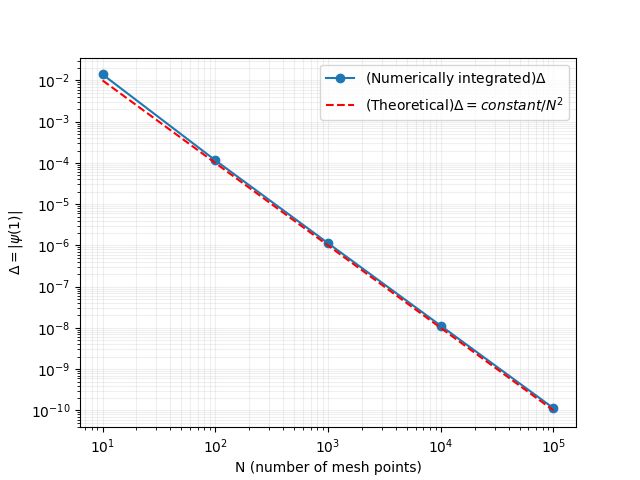
\includegraphics[width=0.7\textwidth]{q1-delta_psi.png}
    % \caption{Log-log plot of $\Delta$ vs $N$.}
    \caption{Log-log plot of $\Delta$ vs $N$. Parameters: $E = 0.5\pi^2$, $N \in \{10, 100, 1000, 10000, 100000\}$, $dx = 1/N$.}
\end{figure}

\textbf{Theory:} The probability of finding the particle at the infinite wall is zero ($\Delta = 0$). 
However Verlet numerical integration introduces an error that decreases quadratically with the number of mesh points $N$. Therefore, we expect $\Delta = \text{constant}/N^2$, which corresponds to a linear relationship in a log-log plot with a slope of roughly $-2$, since $\log(\Delta) = \log(k) - 2 \log(N)$.

\textbf{Results:} The plotted numerical data in the log-log plot shows an approximately linear relationship that is consistent with the theoretical slope of $-2$. This supports the expected quadratic convergence of the Verlet numerical integration method.

\section*{Q2}

\textbf{Method:} We calculate the energy eigenvalues for an infinite box potential (where $V(x)=0$ inside the box and infinite outside). We use a binary search algorithm, paired with the shooting method, with a tolerance of $10^{-9}$ and $N=10000$ mesh points to bracket the 4 lowest energy eigenvalues and plot their respective eigenstates.

\begin{figure}[H]
    \centering
    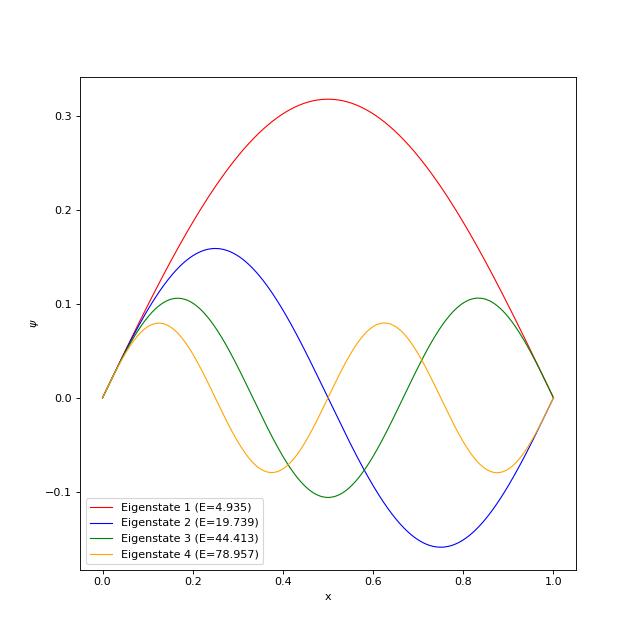
\includegraphics[width=0.7\textwidth]{q2-eigenstate-plots.png}
    % \caption{The 4 corresponding eigenstates for the infinite box potential.}
    \caption{The 4 lowest eigenstates for $V=0$. Parameters: $N=10000$, $dx = 1/N$, tolerance $= 10^{-9}$.}
\end{figure}

\textbf{Theory:} For an infinite box, the theoretical wavefunctions must be exactly 
zero at the boundaries ($\psi(1) = 0$). Furthermore, higher energy states 
possess a larger momentum $p$. 
According to the de Broglie relation $\lambda = \frac{h}{p}$, a larger 
momentum implies a shorter wavelength, leading to more rapid spatial oscillations 
in the wavefunction.

\textbf{Results:} The calculated lowest energy eigenvalues are $E_1 = 4.935, E_2 = 19.739, E_3 = 44.413,$ and $E_4 = 78.957$. The plotted eigenstates show that $\psi(1) \approx 0$ at the boundary. In agreement with the de Broglie theory, we observe that the number of oscillations in the wavefunction increases consistently with the energy state $n$.

\section*{Q3}

\textbf{Method:} We simulate the harmonic oscillator with the potential $V(x) = \frac{1}{2}x^2$ using $N=10000$ mesh points and a spatial step $dx=5/N$. We compute the lowest four energy eigenvalues using the binary search and shooting method, taking advantage of the parity of the solutions.

\begin{figure}[H]
    \centering
    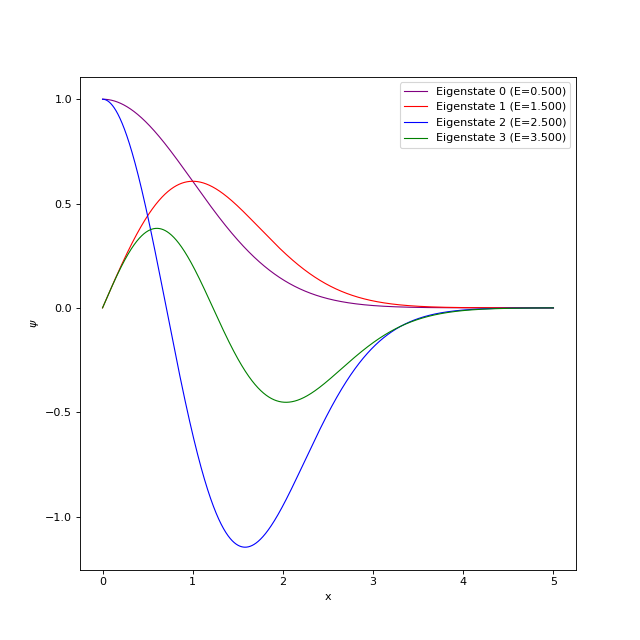
\includegraphics[width=0.7\textwidth]{q3-eigenstate-plots.png}
    % \caption{The 4 lowest eigenstates for the harmonic oscillator.}
    \caption{The 4 lowest eigenstates for the harmonic oscillator. Parameters: $N=10000$, $dx = 5/N$, tolerance $= 10^{-9}$.}
\end{figure}

\textbf{Theory:} The time independent schrödinger equation for the harmonic oscillator is $-\frac{1}{2}\frac{d^2\psi}{dx^2} + \frac{1}{2}x^2\psi = E\psi$. This can be solved analytically using Hermite polynomials $H_n(x)$, yielding the exact solutions $\psi_n(x) = A_n e^{-x^2/2} H_n(x)$ and exact energy eigenvalues $E_n = n + 1/2$. The eigenstates must satisfy parity boundary conditions at $x=0$: even states ($n$ even) have $\psi(0)=1, \psi'(0)=0$, while odd states ($n$ odd) have $\psi(0)=0, \psi'(0)=1$. All physical wavefunctions must decay to zero as $x \to \infty$.

\textbf{Results:} The numerically calculated energy eigenvalues are exactly $E_0 = 0.500, E_1 = 1.500, E_2 = 2.500,$ and $E_3 = 3.500$, which is consistent with the theoretical values $E_n = n + 1/2$. Additionally, the plotted eigenstates visibly satisfy the expected parity conditions at the origin ($x=0$) and correctly decay toward zero at large distances ($x \to 5$).

\section*{Q4}

\textbf{Method:} We calculate the 4 lowest energy eigenvalues for an anharmonic potential $V(x) = \frac{1}{2}x^2 + \frac{1}{2}x^4$. We then compute the theoretical first-order perturbation approximation 
where the unperturbed Hamiltonian is $H_0 = -\frac{1}{2}\frac{d^2}{dx^2} + \frac{1}{2}x^2$ and the 
perturbation is $H_1 = \frac{1}{2}x^4$. 

\begin{table}[H]
    \centering
    \begin{tabular}{ccc}
        \toprule
        $n$ & Numerical $E$ & Perturbation $E$ \\
        \midrule
        0 & 0.696 & 0.875 \\
        1 & 2.325 & 3.375 \\
        2 & 4.328 & 7.375 \\
        3 & 6.579 & 12.875 \\
        \bottomrule
    \end{tabular}
    \caption{Energy eigenvalues for the anharmonic potential.}
\end{table}

\begin{figure}[H]
    \centering
    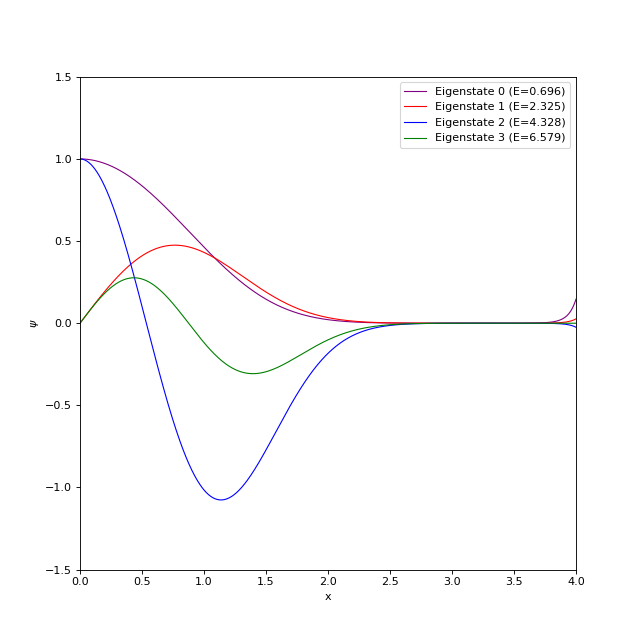
\includegraphics[width=0.7\textwidth]{q4-eigenstate-plots.png}
    % \caption{The 4 lowest eigenstates for the anharmonic potential.}
    \caption{The 4 lowest eigenstates for the anharmonic potential. Parameters: $N=10000$, $dx = 5/N$, tolerance $= 10^{-9}$.}
\end{figure}

\textbf{Theory:} First-order perturbation theory provides the energy correction $E_n^{(1)} = \langle \psi_n^{(0)} | H_1 | \psi_n^{(0)} \rangle$, yielding corrected eigenvalues $E_n \approx E_n^{(0)} + E_n^{(1)}$. This approximation is generally only valid and accurate when the perturbation is relatively small compared to the unperturbed Hamiltonian.

\textbf{Results:} In figure 4, the wave functions decay towards zero (similarly to figure 3) but then start to blow up near $x=4$. The numerical results in 
the table show that the first-order perturbation approximation consistently overestimates the energy eigenvalues. As $n$ increases, the deviation between the numerical 
results and the perturbation method grows significantly. 
% This agrees approximately with theory: the perturbation $V' = x^4/2$ becomes very large for highly excited states (which extend to larger $x$), severely 
% violating the assumption of a "small" perturbation and rendering the first-order approximation inadequate for higher energy levels.

\end{document}
